%Quote

\documentclass{article}
\usepackage{graphicx}
\usepackage[pdftex,bookmarks,bookmarksnumbered,colorlinks]{hyperref}
\usepackage{pdfpages}
\usepackage{fancyhdr}
\usepackage[english]{babel}
\usepackage{multicol}
\usepackage[margin=1.1in]{geometry}
\usepackage{textcomp}
\usepackage{fmtcount}
\usepackage[utf8]{inputenc}
\usepackage{hyperref}

%Prevents Tables from being repositioned
\usepackage{float}
\restylefloat{table}

% Table spacing
%Top space
\newcommand{\Toprule}{\rule{0pt}{3.0ex}}
%Bottom space
\newcommand{\Botrule}{\rule[-1.2ex]{0pt}{0pt}}

%Constants
\newcommand{\DocTitle}{2016 Engineering Consulting Roster Proposal}
\newcommand{\Customer}{The Corporation of the City of Windsor}
\newcommand{\Target}{ }
\newcommand{\Address}{400 City Hall Square East, Suit 403}
\newcommand{\JobNum}{Q7077}


%hyperlinks
\hypersetup{
pdftoolbar=true,        								% show Acrobat�s toolbar?
pdfmenubar=true,        								% show Acrobat�s menu?
pdffitwindow=false,     								% window fit to page when opened
pdfstartview={FitH},    								% fits the width of the page to the window
pdftitle={\DocTitle},    								% title
pdfauthor={PowerCore Engineering},    	% author
pdfsubject={Report},   									% subject of the document
pdfcreator={PowerCore Engineering},   	% creator of the document
pdfproducer={PowerCore Engineering}, 		% producer of the document
pdfnewwindow=true,      								% links in new window
colorlinks=true,       									% false: boxed links; true: colored links
linkcolor=black,          							% color of internal links (change box color with linkbordercolor)
citecolor=blue,        									% color of links to bibliography
filecolor=blue,      										% color of file links
urlcolor=blue}           								% color of external links

%Section Numbering Control
\renewcommand\thesection{\Alph{section}}
%\renewcommand\thesubsection{\arabic{subsection}}
%\renewcommand\thesubsubsection{\arabic{subsubsection}}
%\renewcommand\thesubsubsubsection{\thesection.\thesubsection.\thesubsubsection.\arabic{subsubsubsection}}

%Header and Footer
\renewcommand{\sectionmark}[1]{\markboth{#1}{}}
\renewcommand{\footrulewidth}{0.4pt}
\fancyhead[R]{\leftmark} % 1. sectionname
\fancyfoot[C]{\thepage}
\fancyfoot[L]{
PowerCore Engineering Ltd.\\
London, Ontario, Canada\\
Tel: (519) 474-1175\\
\url{www.powercore.ca}}
\cfoot{ }

\fancyfoot[R]{
\DocTitle \\ \vspace{12pt}  \thesection -\thepage }
\fancypagestyle{plain}{%
  \fancyhf{}%
  \renewcommand{\headrulewidth}{0pt}%
}
\fancyhead[L]{ % right
   
\includegraphics[height=0.4in]{../Images/PCEHeaderLogo.png}
}

\begin{document}

\pagenumbering{roman}
\begin{titlepage}
\thispagestyle{empty}
\center % Center everything on the page

%Title Page Header
\begin{center}

\includegraphics[height=1in, keepaspectratio=true]{../Images/PCEHeader.PNG}
\end{center}

%TITLE SECTION
\begin{center}
\vspace{20mm}
\Huge \DocTitle \\ % Title of your document
\vspace{75mm}
\large Prepared for: \\
\LARGE\textbf{\Customer} \\
\large\textbf{\Building}\\
\small\textbf{\Address}\\
\end{center}


%LOGO SECTION
%
\includegraphics[width=2.5in, keepaspectratio=true]{Images/logo_SV.png} 

 
%AUTHOR SECTION
\begin{flushleft} \large
\vfill

\textbf{Prepared by:} \\
Roman Bulla, P. Eng., Scott Vermeire, EIT \\
%Roman Bulla, P. Eng., Vince Klingenberger \\
\vspace{12pt} 
\textbf{Completion:}\\
\today \\ 
\vspace{12pt} 
\textbf{Job Number:}\\
\JobNum \\
\end{flushleft}

\end{titlepage}


%TOC
\tableofcontents
\pagebreak

\pagenumbering{arabic}
\pagestyle{fancy}

%Submission Contents
%Declaration of Conflict


\section{Offer Documents}
Please review PowerCore Engineering's signed Offer Documents in the following section. 
\includepdf[pages=-]{Offer.pdf}

\section{Submission Contents}
\subsection{Declaration of Conflict}
\label{Sub:DOC}
\subsubsection{Introduction}
\label{Sub:DOC:intro}
PowerCore Engineer Ltd. have read and understood The City of Windsor's policy on declaration of conflicts and have no such conflicts of interest to declare.\\

Such conflicts would include relationships with any person(s) employed by the City in any capacity that:

\begin{enumerate}
	\item having a direct or indirect financial interest in the award of the Contract to any Proponent;
	\item is currently employed by, or is a consultant to or under contract to a Proponent;
	\item is negotiating or has an arrangement concerning future employment or contracting with any Proponent;
	\item has an ownership interest in, or is an officer or director of any Proponent.
\end{enumerate}
\pagebreak
%Proponent Info

\subsection{Proponent Info}
\label{Sub:PI}

\noindent Dear City of Windsor, \\



\noindent Thank you for the opportunity to present our proposal for your Engineering Consulting Roster.\\



\noindent PowerCore Engineering is a Power Distribution Systems Engineering, Maintenance and Testing company based in London Ontario.  Our team consists of electrical engineering and technical professionals with extensive experience in power system engineering, engineered drive systems, power quality and energy demand management.\\ 

\noindent PowerCore Engineering specializes in Power Distribution System Engineering (e.g. Short Circuit, Protective Device Coordination, Ground Grid Analysis and Power Quality Analysis), as well as Design, Managements, Maintenance and Testing of power distribution systems.  \\


Our core competence also includes Power Monitoring and Management Systems, Energy Reporting Programs and Energy and Demand Control Automation systems.  \\


We also have exceptional expertise in Engineered VFD and DC Drive systems for Large Power Applications, as well as special Automation Projects (such as High power VFD systems, Test Stations for large rotating machinery, etc.).\\

\noindent For more info please refer to our page at:  http://www.powercoreeng.com\\

\subsubsection{Certification}
\label{Sub:DOC:cert}
\begin{enumerate}
	\item Authorized by the Association of Professional Engineers of Ontario to offer professional engineering services.
	\item Schneider Power Monitoring and Energy Management Systems Authorized Integrator for Ontario
	\item Yaskawa Drives Integrator for Ontario
	\item IEEE Member
	\item ECRA Licensed
\end{enumerate}

\subsubsection{Location}
\label{Sub:DOC:loc}

\noindent\textbf{PowerCore Engineering Office Location:} \textcolor[rgb]{0,0,0}{\textcolor[rgb]{0,0,1}{4096 Meadowbrook Dr., Unit 133, London, ON;  N6L 1G}}\\
\noindent\textbf{Distance to Windsor City Hall:} \textcolor[rgb]{0,0,1}{184km}\\

 
\pagebreak
%Health, Safety and Workplace Violence and Harassement Acknowledgement

\subsection{Health, Safety and Workplace Violence and Harassment Acknowledgment}
\label{Sub:HS}

\subsubsection{PowerCore Health And Safety Program}
\label{Sub:HS:HSP}

Please review PowerCore Engineering's Health and Safety Program outlined in the following section. 

\includepdf[pages=-]{SignedHealthAndSafetyProgram.pdf}

\subsubsection{Health, Safety and Workplace Violence and Harassment Acknowledgment Form}
\label{Sub:HS:sig}

Please see attached Signed Health, Safety and Workplace Violence and Harassment Acknowledgment Form in the following section. 

\includepdf[pages=-]{AppendixESigned.pdf}

\pagebreak
%Other
\subsection{Other Information}
\label{Sub:OI}

\subsubsection{PowerCore Engineering Employee Curriculum Vitae}
\label{Sub:OI:CVs}

Please review PowerCore Engineering's Employee Curriculum Vitae outlined in the following section.

\includepdf[pages=-]{PowercoreEngineeringEmployeeCVs.pdf}

\pagebreak

%Experience in Relevant Category
\subsection{Experience in Relevant Category}
\label{Sub:Exp}

\noindent At PowerCore Engineering we specialize in all facets of Power Distribution Engineering and have achieved much success with both public and private clients in institutional, industrial and commercial sectors.  Our only experience with public entities is with the Corporation of the City of London and we have been working with them since 2007.  As stated before, PowerCore Engineering has dealt with a variety of different customers and has provided solutions for the following types of projects.

\subsubsection{Power System Studies}
\label{Sub:Exp:PSS}

%\subsubsubsection{Description}
%\label{Sub:Exp:PSS:Desc}
\textbf{Description}\\
\\
PowerCore Engineering provides an extensive line-up of Professional Electrical Engineering services ranging from simple short circuit and protective coordination studies to complex power system modeling and system design. Some common wide range services for existing power systems are:
\begin{itemize}
	\item Short Circuit Evaluation and Protective Coordination Studies (typically required for all new installations, and advisable after substantial system alterations). This study is performed to evaluate and stipulate the settings for all protective devices including breakers, protective relays, fuses, motor protectors, etc. The results of which ensure optimum system protection in case of fault, i.e. the system branch is safely and selectively isolated before any damage to the system is sustained
	\item Load Flow and Voltage Stability Studies (voltage fluctuation projections, equipment loading assessments, etc.)
	\item Motor Starting Studies and Simulations (most often performed before large motor installations)
	\item Harmonic Analysis (PQ evaluation, capacitor impact forecast, harmonic filters design/specifications, etc.)
	\item Insulation Coordination Studies (HV and MV installations)
	\item Emergency Backup System Audits (power outage impact evaluations, backup system performance, generator/ATS sizing, power system tie-in considerations, etc.)
\end{itemize}


In addition, services for new power distribution systems are provided:
\begin{itemize}
	\item Power System Design for Industrial and Commercial Facilities (drawings, engineering specifications, ESA submittals, contractor liaisons)
	\item Emergency Backup System Design (generators, Automatic Transfer Switches, power system tie-in considerations, etc.)
	\item Ground Grid Design (new and existing substations)
\end{itemize}

%\subsubsubsection{Experience}
%\label{Sub:Exp:PSS:Exp}
\textbf{Experience}\\
\begin{itemize}
	\item PowerCore provides Arc Flash Hazard Analysis for all customers listed in the \hyperref[Sub:Ref]{references} section, as well as, The University of Western Ontario, Fanshawe College, Electro-Motive Diesel and a number of others. 
	\item Specifically for the City of London and Wilfrid Laurier University, PowerCore has annual contracts to analyze facilities with and without Arc Flash Analysis; Running full analysis on facilities that require analysis and updating those that are out of date. In many cases additional protective device coordination studies are typically conducted to maintain selectivity and reduce the arc flash hazard through means of circuit protection adjustments. 
	\item PowerCore has also provided load flow analysis and motors starting studies for companies like Enbridge Pipeline and Henry Company Canada in order to troubleshoot power quality issues and to optimize transformer on-load tap changers.

\end{itemize}

\subsubsection{Power Quality Analysis}
\label{Sub:Exp:PQA}

%\subsubsubsection{Description}
%\label{Sub:Exp:PQA:Desc}
\textbf{Description}\\
\\	
Power Quality is often called into question but, be it simple Power Factor correction capacitors or a complex harmonic filtering system, there is a solution to fit any budget or schedule.\\ 

PowerCore's in-house expertise along with its partners can resolve commonly experienced issues such as:
\begin{itemize}
	\item Excessive Harmonic Distortion
	\item Sub Cycle Transients
	\item Voltage Flicker
	\item Voltage Fluctuation
	\item Neutral Cable Overheating
	\item Ground Loops/Grounding Problems
\end{itemize}

In addition, complex PQ Audits can be provided that will assess the entire facility power distribution system from the top down. Typically, power quality is evaluated through a Power Monitoring System (if the facility has one) or a series of Power Quality Measurements are performed. \\

PowerCore Engineering can provide such customized PQ Solutions as:
\begin{itemize}
	\item Fixed PF Correction Capacitor Banks
	\item Switched-in Capacitor Banks
	\item Harmonic Filters
	\item Voltage Regulators
	\item K-rated Transformers
	\item TVSS
\end{itemize}


%\subsubsubsection{Experience}
%\label{Sub:Exp:PQA:Exp}
\textbf{Experience}\\
\begin{itemize}
	\item PowerCore Engineering has designed site specific condition filters for Panabrasive Inc, GM CAMI Assembly, Atlas Copco and a number of others.
	\item PowerCore has installed and/or retrofitted power factor correction capacitor banks for a number of site such as The city of London, Great Lakes Copper, The Original Cakerie, Fischer Canada and a number of others. PowerCore has installed these capacitor banks in an economical manner with 2-3 year payback periods.
	\item PowerCore Engineering has specified and installed various TVSS for Wilfrid Laurier University and Great Lakes Copper in order to add reliable surge protection.  
\end{itemize}

\subsubsection{Portable Power Monitoring}
\label{Sub:Exp:PowM}

%\subsubsubsection{Description}
%\label{Sub:Exp:PowM:Desc}
\textbf{Description}\\
\\
Whether or not a Power Monitoring System is installed in the facility there is occasional need to perform on-the-spot power measurements to evaluate particular load parameters such as:
\begin{itemize}
	\item Load Flow
	\item Voltage Sags and Swells
	\item Power Factor
	\item Power Quality
\end{itemize}
Local power measurements are typically required if there is a need to:
\begin{itemize}
	\item Assess loading of a selected feeder(s)
	\item Decide whether particular feeders can accept large load additions
	\item Measure Harmonic Distortion when the power quality of the supply is in question
	\item Provide Power Factor compensation for a facility or locally to release capacity
	\item Calculate the projected impact of large load installation
\end{itemize}

Our Portable Power Monitoring Package based on PML ION 7500 meter provides all the necessary information within moments. The power monitors are typically installed in customer specified locations for a period of 1-7 days, but other arrangements are possible. When installing the power monitor power interruption is usually not required.

%\subsubsubsection{Experience}
%\label{Sub:Exp:PowM:Exp}
\textbf{Experience}\\
\begin{itemize}
	\item PowerCore has supplied and installed temporary power monitors in a number of locations.  Such locations include site for the city of London, Black Fly, Sealed Air, Electro-Motive Diesel, Formosa Springs Brewery, Great Lakes Copper, General Dynamics Land Systems and a number of others.
\end{itemize}

\subsubsection{Power Monitoring and Energy Management Systems}
\label{Sub:Exp:PM}

%\subsubsubsection{Description}
%\label{Sub:Exp:PM:Desc}
\textbf{Description}\\
\\	
An electrical power distribution system is the crucial backbone of any facility. In today's industrial environment there are a few pivotal demands on electrical systems. 
\begin{itemize}
	\item Reliability of supply
	\item Cost control and allocation
	\item Power quality monitoring and assurance
\end{itemize}

Power monitoring and energy management systems enable full overview and insight into existing and historical energy consumption. With the right implementation this information can be accessible anywhere and at any time.\\ 

Existing power monitoring equipment may already be installed in the facility. In many cases only a small step is required to bring this available data into an Energy Management System. By having an Energy Management System it allows for a centralized approach to monitor and analyze Water, Air, Gas, Electricity, and Steam (W.A.G.E.S.) data. \\

PowerCore Engineering can provide customized Energy Management solutions by: 
\begin{itemize}
	\item Utilizing existing communication-ready power meters
	\item Adding new power monitors in selected locations
	\item Working on different hardware platforms by combining power meters by leading manufacturers
	\item Providing Central Energy Management software to integrate all remote meters and integrate it in the existing Building/Process management system
	\item Providing customized reporting tools based on SQL database and/or MS Excel TM
	\item Web-based remote control and monitoring

\end{itemize}


Decisions on location of electrical supply for large equipment or analysis of the financial impact of production schedules is made easy. The benefits of service from PowerCore Engineering are clear in Power Monitoring whether a stand alone digital meter or a fully integrated Internet-ready Energy Management system is needed. 

%\subsubsubsection{Experience}
%\label{Sub:Exp:PM:Exp}
\textbf{Experience}\\
\begin{itemize}
	\item PowerCore Engineering has serviced and installed power monitoring systems in such facilities as The City of London, Wilfrid Laurier University, Great Lakes Copper, McMaster University, Presstran, ESSO IOL, Electro-Motive Diesel, General Dynamics London, Liberty Freezers, The University of Wester Ontario and a number of others.
	\item Although PowerCore Engineering is a certified integrator for Schneider ION meters, PowerCore possess the skills and experience to work with any brand of Power Monitoring equipment.
\end{itemize}


\subsubsection{Power System Maintenance}
\label{Sub:Exp:PSM}

%\subsubsubsection{Description}
%\label{Sub:Exp:PSM:Desc}
\textbf{Description}\\
\\	 
Keeping power distribution systems up to standard requires periodic electrical testing and maintenance programs to be in place (see International Electrical Testing Association's article on the issue: Frequency of Maintenance Tests) Generally, 1-3 year testing frequency is advisable depending on the age and condition of the equipment. \\

Even if a periodic maintenance and testing program is in place, the resources or time to manage and oversee an effective economic testing program may not be available. PowerCore can perform the electrical maintenance and testing, or act as consultants on the design, implementation, and oversight of the electrical testing and maintenance. \\

PowerCore has an extensive experience in field testing electrical power distribution equipment and is able to: 
\begin{itemize}
	\item Devise an effective electrical testing program
	\item Prepare testing specifications and schedules
	\item Eliminate unnecessary testing (frequency and scope)
	\item Assist in selecting testing agencies or contractors
	\item Ensure that the selected testing agency performs the work as outlined
	\item Review the results of the tests and recommend actions only as necessary
\end{itemize}

Having PowerCore Engineering as an acting consultant saves money in the long term by reducing maintenance cost without sacrificing effectiveness. Not only is it ensured that any problems encountered are dealt with in a timely and effective manner, but also that a fair price is paid for only the components needed.

%\subsubsubsection{Experience}
%\label{Sub:Exp:PSM:Exp}
\textbf{Experience}\\
\begin{itemize}
	\item PowerCore Engineering has annual maintenance contracts with all the customers listed in the \hyperref[Sub:Ref]{references} section.  Other customers PowerCore has provided maintenance services for, outside of the reference list, include: Great lakes Copper, Meritor Suspension Systems Company (MSSC), ESSO IOL, Electro-Motive Diesel, London District Energy and a number of others.
\end{itemize}

\subsubsection{Switchgear Retrofit }
\label{Sub:Exp:SR}

%\subsubsubsection{Description}
%\label{Sub:Exp:SR:Desc}
\textbf{Description}\\
\\
When extra time must be squeezed from existing power distribution system components or there are concerns regarding the safety of existing equipment, PowerCore, together with partners, can offer such customized services as: 
\begin{itemize}
	\item HV and LV Switchgear Revamp (on-site repairs, OEM and third party replacement components
	\item Breaker Retrofit (protective trip unit replacement, charging/closing/tripping mechanism replacement, etc.)
	\item HV ad MV Relays Replacement (analogue relays replacement with the digital equivalent, protection scheme upgrades)
	\item MV and LV Contractor Retrofit (starter cubicle overhaul, protection upgrade)

\end{itemize}

Together with its partners, PowerCore Engineering provides services to extend life expectancy of existing power systems by offering economical re-building of electrical system components, thus ensuring safe and reliable operation.

%\subsubsubsection{Experience}
%\label{Sub:Exp:SR:Exp}
\textbf{Experience}\\
\begin{itemize}
	\item PowerCore has provided engineering and rebuild services for Ingredion (formerly CASCO) and Great Lakes Copper in order to facilitate new high voltage equipment while maximizing space efficiency and infrastructure previously in place.
	\item For Bell Canada and Meritor Suspension Systems Company (MSSC), PowerCore has overhauled and upgraded old circuit breaks and trip units in order to extend life and provide reliability. 
\end{itemize}

\subsubsection{Ground Fault Alarm and Location Systems}
\label{Sub:Exp:SR}

%\subsubsubsection{Description}
%\label{Sub:Exp:SR:Desc}
\textbf{Description}\\
\\
Since Ground Faults represent 90\% of all electrical faults an effective and quick Ground Fault detection system is vital to all facilities. \\

Ground indicator lights are the minimum requirement of the Canadian Electrical Code (Rule 10-106 (2) ). This is by no means an ideal setup since they require daily inspection. Ideally, Power Monitoring systems are used to send email, page, or SMS messages to the appropriate people to deal with the issue. \\

PowerCore Engineering supplies, installs, and commissions the Neutral Voltage and Current Monitoring system on any distribution system as follows: 
Installs a current monitoring CT and voltage monitoring circuit and ties them either into an existing energy management system or supplies and installs a suitable power monitor\\


Configures the Power Monitor and the Energy Managemnt software to alarm on neutral to ground voltage and neutral current present. The alarm can be displayed using the energy management software or any other SCADA/HMI system present in the facility.\\

Configures the Energy Management Server to launch an external alarm program to email or page appropriate personnel.\\

Once a ground fault is detected, it is advisable to clear it as soon as possible. Locating a ground fault is a task that can dishearten any electrician and can be a time consuming and frustrating task which may require shutting down vital equipment and disruption of the power supply. \\

An alternative non-disruptive method of locating a ground fault within the system is to implement a pulsating ground current concept.\\

A parallel grounding resistor is inserted into the circuit via a pulsating relay that operates at a predefined frequency.\\

A large probe is then applied around a set of three phase conductors at different power feeders and connected to a suitable DMM.\\

The feeder that has a ground fault on it will display a pulsating signal at a predefined frequency, thus narrowing down the ground fault search (see \hyperref[htbp]{diagram}).\\

\begin{figure}[htbp]
	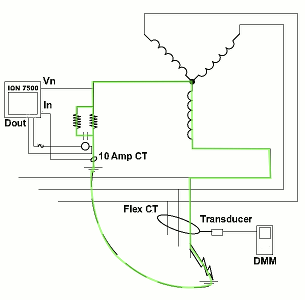
\includegraphics[height=4in]{../Images/locator-diagram.png}

	\caption{Ground Fault Detection System}
	\label{fig:GroundFaultDetectionSystem}
\end{figure}

%\subsubsubsection{Experience}
%\label{Sub:Exp:SR:Exp}
\textbf{Experience}\\
\begin{itemize}
	\item PowerCore Engineering has implemented several systems at Presstran, Electro-Motive Diesel, General Dynamics and others.
\end{itemize}

\subsubsection{Variable Frequency Drive (VFD) Applications}
\label{Sub:Exp:VFD}

%\subsubsubsection{Description}
%\label{Sub:Exp:VFD:Desc}
\textbf{Description}\\
\\
Motor Starter and Variable Frequency Drive applications range from a simple stand alone starter application to a full blown Starter/VFD/Bypass system. On the VFD side, most applications require careful sizing of the system components as well as proper feature selection (Vector/Frequency/Servo control VFD, external references, communication, etc.). The starter applications (across-the-line or soft-start with a bypass) typically present complications only when large motors are involved (200 HP and higher). In such cases, a system simulation to assess large motor starting current effects is advisable to avoid voltage stability problems in the facility. 

PowerCore Engineering helps with such aspects of independent Customized VFD/Starter Application as: 
\begin{itemize}
	\item VFD/Starter selection based on process requirement
	\item System simulation of the large starter application (across-the-line vs. Soft-start)
	\item Line/Load reactors for VFD selection
	\item Drive/Starter supply, installation, and programming
	\item External control interface (Digital and Analogue controls)
	\item Communication interface to external SCADA or energy management systems
	\item Control and interface drawings
\end{itemize}

A VFD or a soft starter installed can be a very effective and economical way to control large motor loads. Having it properly sized and selected can avoid many problems and pitfalls that may be associated with such an application.

%\subsubsubsection{Experience}
%\label{Sub:Exp:VFD:Exp}
\textbf{Experience}\\
\begin{itemize}
	\item PowerCore Engineering as provided turn key multi winder drive systems for AEP Canada.
	\item PowerCore Engineering designed and built multiple 14 VFD Motor Control Centers for Goldcorp.
	\item PowerCore Engineering has been designing and servicing both AC and DC motor test stations for Electro-Motive Diesel and Progress Rail in both the United States and Mexico. 
	\item PowerCore Engineering has also provided VFD engineering, installation, integration and/or troubleshooting for the City of London, IPEX, Cementation, Natra, Goldcrop and others.
\end{itemize}
	
\subsubsection{Power/Control System Troubleshooting }
\label{Sub:Exp:SR}

%\subsubsubsection{Description}
%\label{Sub:Exp:SR:Desc}
\textbf{Description}\\
\\
Outdated drives or motor starters, a customized control system or a specialized I/O rack breakdown wreaks havoc on any production schedule. Moreover, if the original supplier or installer is not available small failures easily morph into huge problems if the solutions are not administered promptly. 

PowerCore offers help in such cases with: 
\begin{itemize}
	\item On-site/Off-site troubleshooting and repair of industrial and commercial electrical and electronic equipment
	\item Reverse engineering (re-constructing system drawings and operation manuals in the absence of the original documentation)
	\item Outdated and rare equipment sourcing
	\item Replacement of obsolete parts with up-to-date equivalents
	\item Re-design and supply installations for unrepairable components or systems
\end{itemize}

%\subsubsubsection{Experience}
%\label{Sub:Exp:SR:Exp}
\textbf{Experience}\\
\begin{itemize}
	\item PowerCore has also performed troubleshooting and recommissioning of sophisticated protections systems on Harvest Power and London District Energy's multi generator cogen system.
	\item PowerCore has also serviced many  troubleshooting
\end{itemize}

\subsubsection{Tender Preparation}
\label{Sub:Exp:TP}

%\subsubsubsection{Description}
%\label{Sub:Exp:TP:Desc}
\textbf{Description}\\
\\
When new power distribution systems are planned or in a stage of preliminary design, PowerCore offers services such as:
\begin{itemize}
	\item Power System Design new systems or additions for Industrial or Commercial Facilities (drawings, engineering specifications, submittable, contractor liaison)
	\item Emergency Backup System Design (generator, Automatic Transfer Switch, power system tie-in considerations, etc.)
	\item Ground Grid Design (new and existing substations)
\end{itemize}
Once the system design is in place, it is possible to assist with project tender process management in several ways by:
\begin{itemize}
	\item Preparing complete tender packages for bid submittable (outlining contractor/customer responsibilities, ensuring/obtaining ESA approvals, reviewing drawings and specifications, etc.)
	\item Organizing tender meetings (with customer representatives, contractors, utility representatives, etc.)
	\item Assisting in bid evaluations (examining contractor bids, assessing compliance, clarifying scope, consulting with suppliers and contractors)
	\item Supervising project realization (supervising installations and commissioning, ensuring all requirements are fulfilled, acting as a customer-contractor liaison, day-to-day matters)
	\item Verifying final submittable (equipment manufacturer submittable, contractor submittable, commissioning reports, ESA inspections)

\end{itemize}
%\subsubsubsection{Experience}
%\label{Sub:Exp:TP:Exp}
\textbf{Experience}\\
\begin{itemize}
	\item 	
	\item Emergency Backup System Audits (power outage impact evaluations, backup system performance, generator/ATS sizing, power system tie-in considerations, etc.)

\end{itemize}
	
\pagebreak
%Proponent Qualifications in Relevant Category
\subsection{Proponent Qualifications in Relevant Category}
\label{Sub:Qual}

Please review PowerCore Engineering's Project Assignment Personnel Profile outlined in the following section.

\includepdf[pages=-]{Profile.pdf}

%References
\subsection{Reference}
\label{Sub:Ref}

Please review PowerCore Engineering's Reference Information outlined in the following section. 

\includepdf[pages=-]{Reference.pdf}






\end{document}